\documentclass{article}
\usepackage[utf8]{inputenc}
\usepackage[a4paper, top=2cm, bottom=2cm, left=2cm, right=2cm]{geometry}
\usepackage{amsfonts}
\usepackage{amsmath}
\usepackage{amssymb}
\usepackage{amsthm}
\usepackage{esint}
\usepackage{fancyhdr}
\usepackage{enumitem}
\usepackage{amsmath}
\usepackage{amsthm}
\usepackage{amssymb}
% \usepackage{mathabx}
\usepackage[linesnumbered , ruled , vlined]{algorithm2e}
\usepackage{listings}
\usepackage{xcolor}
\usepackage{floatrow}
\usepackage{graphicx}
\usepackage{fancyhdr}
\usepackage{listings}
\usepackage[hypcap=false]{caption}
\usepackage{hyperref}
\usepackage{subfig}
\usepackage{tikz}
\usepackage{hyperref}

\pagestyle{fancy}
\fancyhf{}
\lhead{200050107, 200050130, 200050154, 200050157}
\rhead{CS337}
\cfoot{\thepage}

\newcommand{\B}[1]{\textbf{#1}}
\newcommand{\I}[1]{\textit{#1}}
\newcommand{\norm}[1]{\left\lVert#1\right\rVert}

\title{\textbf{CS337 Course Project \\ Face Recognition}}
\author{Pranjal Kushwaha, Shashwat Garg, Vedang Asgaonkar, Virendra Kabra}
\date{Autumn 2022}

\begin{document}
\begin{sloppypar}       % for overfull, etc.

    \maketitle
    \tableofcontents

    \newpage

    \section{Dataset}
    
        \begin{itemize}
            \item We use the Labelled Faces in the Wild (LFW) dataset. It has been taken from \href{https://www.kaggle.com/datasets/jessicali9530/lfw-dataset}{Kaggle}. There is an uneven distribution of images, with only 10 people having at least 53 images. Thus, we train the model to classify these 10 people, with our dataset containing 53 images for each.
            \item The train-test split is 80-20, and the train set is further split to create the validation set. Equal splits are created for each class.
            \item \B{Data Augmentation}: We add horizontally flipped images to the dataset. This acts as a regularizer, helping the model to generalize better.
        \end{itemize}
    

        \section{Model Architecture}

        We use a Convolutional Neural Network (CNN) to create a multi-class image classifier. The network is inspired from FaceNet \cite{facenet}.

        \begin{center}
            \begin{table}[!h]
                \begin{tabular}{|c|c|c|c|c|}
                    \hline
                    \B{Layer} & \B{In} & \B{Out} & \B{Kernel} & \B{Params}\\
                    \hline \hline
                    conv1 & $250\times 250\times 3$ & $123\times 123\times 64$ & $7\times 7\times 3, 2$ & 9K\\
                    batchnorm1 & $123\times 123\times 64$ & $123\times 123\times 64$ & & 128\\
                    relu1 & $123\times 123\times 64$ & $123\times 123\times 64$ & & 0\\
                    maxpool1 & $123\times 123\times 64$ & $61\times 61\times 64$ & $2\times 2\times 64, 2$ & 0\\
                    dropout1 & $61\times 61\times 64$ & $61\times 61\times 64$ & & 0\\
                    \hline
                    conv2 & $61\times 61\times 64$ & $61\times 61\times 128$ & $3\times 3\times 64, 1$ & 74K\\
                    batchnorm2 & $61\times 61\times 128$ & $61\times 61\times 128$ & & 256\\
                    relu2 & $61\times 61\times 128$ & $61\times 61\times 128$ & & 0\\
                    maxpool2 & $61\times 61\times 128$ & $30\times 30\times 128$ & $2\times 2\times 128, 2$ & 0\\
                    dropout2 & $30\times 30\times 128$ & $30\times 30\times 128$ & & 0\\
                    \hline
                    conv3 & $30\times 30\times 128$ & $30\times 30\times 256$ & $3\times 3\times 128, 1$ & 295K\\
                    batchnorm3 & $30\times 30\times 256$ & $30\times 30\times 256$ & & 512\\
                    relu3 & $30\times 30\times 256$ & $30\times 30\times 256$ & & 0\\
                    maxpool3 & $30\times 30\times 256$ & $15\times 15\times 256$ & $2\times 2\times 128, 2$ & 0\\
                    dropout3 & $15\times 15\times 256$ & $15\times 15\times 256$ & & 0\\
                    \hline
                    conv4 & $15\times 15\times 256$ & $15\times 15\times 64$ & $3\times 3\times 256, 1$ & 148K\\
                    batchnorm4 & $15\times 15\times 64$ & $15\times 15\times 64$ & & 128\\
                    relu4 & $15\times 15\times 64$ & $15\times 15\times 64$ & & 0\\
                    dropout4 & $15\times 15\times 64$ & $15\times 15\times 64$ & & 0\\
                    \hline
                    flatten & $15\times 15\times 64$ & 14400 & & 0\\
                    \hline
                    fc1 & 14400 & 1024 & & 14M\\
                    relu5 & 1024 & 1024 & & 0\\
                    dropout5 & 1024 & 1024 & & 0\\
                    \hline
                    fc2 & 1024 & 64 & & 66K\\
                    relu5 & 64 & 64 & & 0\\
                    dropout5 & 64 & 64 & & 0\\
                    \hline
                    fc3 & 64 & 10 & & 650\\
                    \hline \hline
                    Total & & & & 15M\\
                    \hline
                \end{tabular}
                \caption{\label{table-1}Model Architecture}
            \end{table}
        \end{center}

        Notation for kernels: Size $\times$ Number of channels, Stride.

        \begin{itemize}
            \item \B{Convolutions}: To learn hierarchical representations of the input data, we use several convolutional layers. Given input of size $(N, C_{in}, H_{in}, W_{in})$ and output of size $(N, C_{out}, H_{out}, W_{out})$, the output value is
                $$ out(N_i,C_{out_j}) = \sum_{k=0}^{C_{in}-1} W(C_{out_j},k) \ast input(N_i,k) + b(C_{out_j}) $$
            where $\ast$ denotes cross-correlation (flipped convolution), $N$ is the batch size, $C$'s are the number of channels, $H$ and $W$ are heights and widths. The parameters $W$ and $b$ are trainable. Cross-correlation is used to avoid flipping the filters. Since the weights are \I{learnt}, this is equivalent to using convolution.
            \item Batch Normalization: Adding these layers lead to faster convergence.
            \item ReLU: These are added for non-linearity, which is necessary for the universal approximation theorem to hold. The operation $ReLU(x)=\max(0,x)$ is applied element-wise.
            \item Max Pooling: Pooling involving down-sampling the feature maps by summarizing the features. In particular, max pooling outputs the maximum of input values over the specified region. This also helps make the representation become approximately invariant to small translations of the input.
            \item Dropout: It refers to dropping out random (non-output) neurons in the network, to prevent units from co-adapting too much. This prevents overfitting, thus acting as a regularizer. We use dropout with $p=0.2$ after the maxpool layers \cite{dropout_analysis}, and with $p=0.5$ after the fully-connected layers \cite{dropout_hinton}.
            \item Optimizer: Stochastic Gradient Descent (SGD) is used
                \begin{itemize}
                    \item Learning Rate: $10^{-3}$ is used. Convergence is achieved in less than 50 epochs. In comparison, smaller learning rates (order $10^{-4}$) require many more epochs.
                    \item Weight Decay: $10^{-3}$ is used. For SGD, this is equivalent to using $L_2$ regularization.
                \end{itemize}
            \item Loss: We use two losses in addition:
                \begin{itemize}
                    \item Cross Entropy Loss: This is the standard loss for multi-class classification.
                    \item Triplet Loss: This loss encourages clustering in the latent representation. It is described in a later section.
                \end{itemize}
        \end{itemize}

    
    \section{Dataset Modification Handling}

    As per the usecase, this model might require frequent updation of the faces/people in the dataset. An example can be updating the employee list in the company, where this system is used for attendance.

    For this reason, we have designed our model as an encoder-decoder system. The majority of parameters are in the encoder model and only the final layer is present as a decoder. The idea is that we only need to retrain only the final layer whenever the dataset gets updated.

    This kind of transfer learning results in much quicker learning everytime the dataset is updated. We also see similar validation accuracy levels reached after retraining, upon increasing the dataset's size.

    \section{Comparison with VGG16}

    We also trained a VGG16 model for face recognition using the dataset and limited resources we had. The VGG system was a much deeper Neural Network with several convolution layers and was slow to train. After 500 epochs, we saw the VGG system reach $70\%$ test accuracy. It was improving at a very slow pace.
    
    On the other hand, our model achieves a much better test accuracy of near $90\%$ within 30 epochs with a much smaller training time.

    We conclude that our model outperforms the VGG16 model in case of limited resources and time.


    \section{Analysis}

    \begin{itemize}
        \item Batch Size
            \begin{center}
                \begin{minipage}[b]{0.3\linewidth}
                    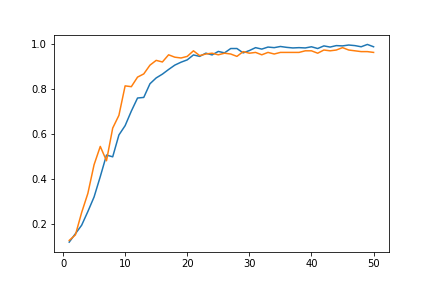
\includegraphics[width = \linewidth]{analysis/batch_size/b=1/b=1.png}
                    \captionof{figure}{Batch Size 1}
                \end{minipage}
                \hfill
                \begin{minipage}[b]{0.3\linewidth}
                    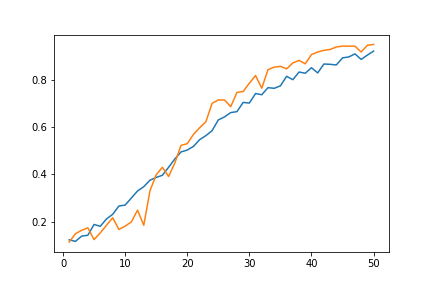
\includegraphics[width = \linewidth]{analysis/batch_size/b=5/b=5.png}
                    \captionof{figure}{Batch Size 5}
                \end{minipage}
                \hfill
                \begin{minipage}[b]{0.3\linewidth}
                    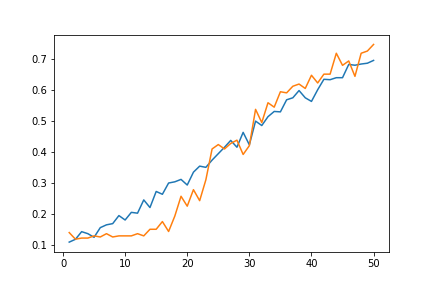
\includegraphics[width = \linewidth]{analysis/batch_size/b=10/b=10.png}
                    \captionof{figure}{Batch Size 10}
                \end{minipage}
            \end{center}
            A batch size of 1 leads to better and faster convergence.
        \item Batch Normalization
            \begin{center}
                \begin{minipage}[b]{0.45\linewidth}
                    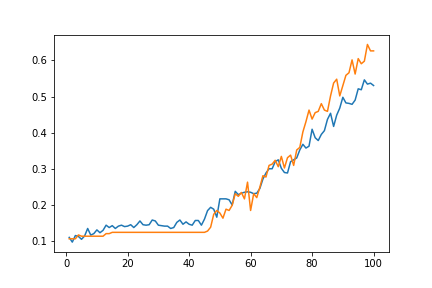
\includegraphics[width = \linewidth]{analysis/batchnorm/without/without.png}
                    \captionof{figure}{Without Batch Norm}
                \end{minipage}
                \hfill
                \begin{minipage}[b]{0.45\linewidth}
                    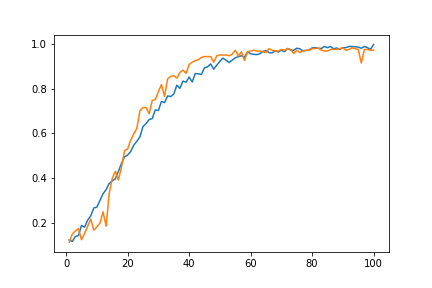
\includegraphics[width = \linewidth]{analysis/batchnorm/with/withbatchnorm.png}
                    \captionof{figure}{With Batch Norm}
                \end{minipage}
            \end{center}
            Faster convergence is observed with batch normalization.
            \item Optimizer
            \begin{center}
                \begin{minipage}[b]{0.45\linewidth}
                    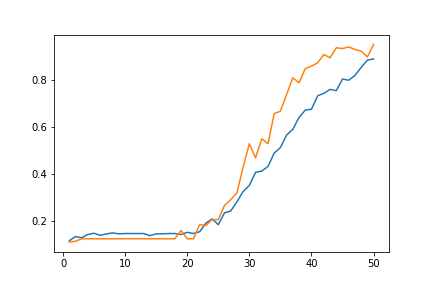
\includegraphics[width = \linewidth]{analysis/optimizer/adam/adam.png}
                    \captionof{figure}{Adam}
                \end{minipage}
                \hfill
                \begin{minipage}[b]{0.45\linewidth}
                    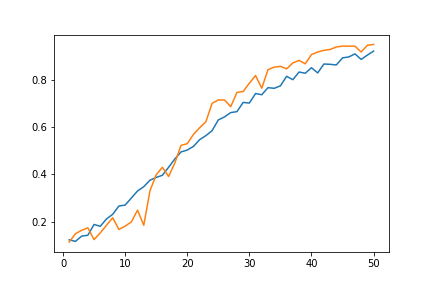
\includegraphics[width = \linewidth]{analysis/optimizer/sgd/sgd.png}
                    \captionof{figure}{SGD}
                \end{minipage}
            \end{center}
    \end{itemize}

    \section{Interpretable Architecture}
    Alongside the categorical cross entropy loss, we use the triplet loss as introduced in FaceNet \cite{facenet}. We view the neural network as an encoder-decoder combination.
    The network upto its penultimate layer is the encoder and the last layer is the decoder. Thus the encoder produces a $64$ dimensional latent representation of each image. 
    The triplet loss encourages clustering in this latent space i.e. the latent representations of images in the same class are close together.
    \par The triplet loss $L_T$ defined on a batch of latent vectors $F$ is given by 
    \begin{equation*}
        L_T(F) = \sum_{f_a \in F} \sum_{f_p \in F_p(f_a)} \sum_{f_n \in F_n(f_a)} [ ||f_a - f_p||^2 - ||f_a - f_n||^2 + \alpha ]_+
    \end{equation*}
    where $F_p(f_a)$ is the subset of $F$ having the same class as $f_a$, $F_n(f_a)$ is its complement and $\alpha$ here is margin which we set to $1$.
    \par Thus, the loss forces latent vectors of the same class to reduce their Euclidean distance, while increasing the Euclidean distance between vectors of different classes.
    \par By employing the triplet loss, the latent vectors get clustered, as measured by the ratio of mean squared distance within a cluster to the mean squared distance between clusters.
    This ratio goes down to roughly $0.3$ by employing the triplet loss.

    \section{Adversarial attack on the CNN}
    We demonstrate an attack on the CNN, in which we provide images which are visually similar to the original image, but get misclassified. To that end, we train a generator which is designed to fool
    the model. The generator adds a bias to each pixel of the image. We first freeze the model weights. The output of the generator is passed to the model as input. We train this composite system using a loss 
    which is negative of the cross entropy loss. This encourages the generator to produce images which are misclassified. We also add a regularizer, to encourage similarity of the generated image with the original one.
    \begin{center}
        \ffigbox [ 1 \textwidth ]{ \caption{Adversarial attack} } { 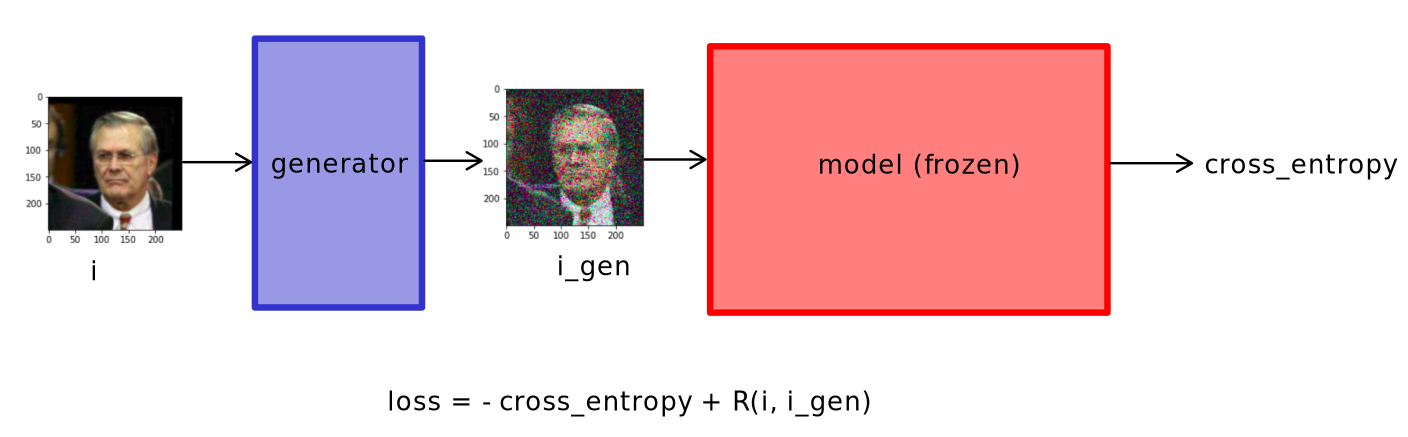
\includegraphics [ width =1 \textwidth ] {attack.png}}   
    \end{center}
    \par Observations:
    \begin{itemize}
        \item By adding a $l_2$ regularizer with $\lambda = 20000$, the generator brings down the model's test accuracy to $35$\% with minimal loss of visual similarity.
        \item $l_1$ regularizer does not do perform as good as $l_2$. Trained with $\lambda = 100$, it brings down the test accuracy to $38$\% but ends up adding too much noise.
    \end{itemize}
    \begin{center}
        \ffigbox [ 0.6 \textwidth ]{ \caption{l1 regularizer} } { 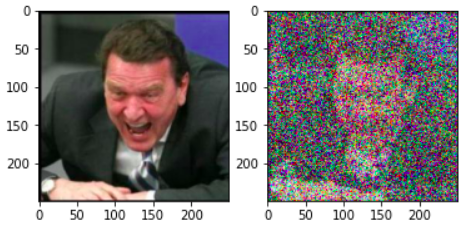
\includegraphics [ width =0.6 \textwidth ] {l1.png}}   
    \end{center}
    \begin{center}
        \ffigbox [ 0.6 \textwidth ]{ \caption{l2 regularizer} } { 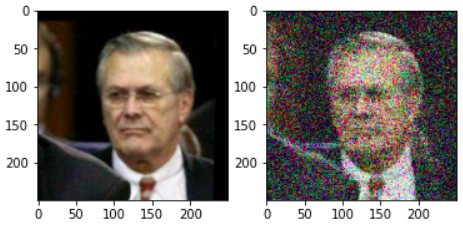
\includegraphics [ width =0.6 \textwidth ] {l2.png}}   
    \end{center}


    \bibliographystyle{abbrv}
    \bibliography{biblio}

\end{sloppypar}
\end{document}